\section{Architectural Views for Suggestions to Improve the Existing System}

\subsection{Context View}

\subsubsection{Stakeholders' Uses of This View}

This perspective provides an overview of the system's context, including the actors and other related systems in a general manner. Website maintainers and data collections of Afetbilgi primarily utilize this view to gain a better understanding of how different actors interact within the website and the system's relationship with external entities like AWS components and the Maps API component.

\subsubsection{Context Diagram}

\afetbilgi is not part of a more extensive system. It is a standalone and open-source efforted website to verify critical information in the fight against the 6 February 2023 Pazarcik Earthquake and deliver it to disaster victims and those who want to help in an understandable, concise manner in multiple languages.

This information is presented in either the form of legible tables with third-party governmental and private links or an interactable method via a map view interface. If deemed necessary, admin and maintainers can make changes to display newly created or edited data and upload it to the system upon any complaints or suggestions they may get on their contact details.

\begin{figure}[H]
  \centering
  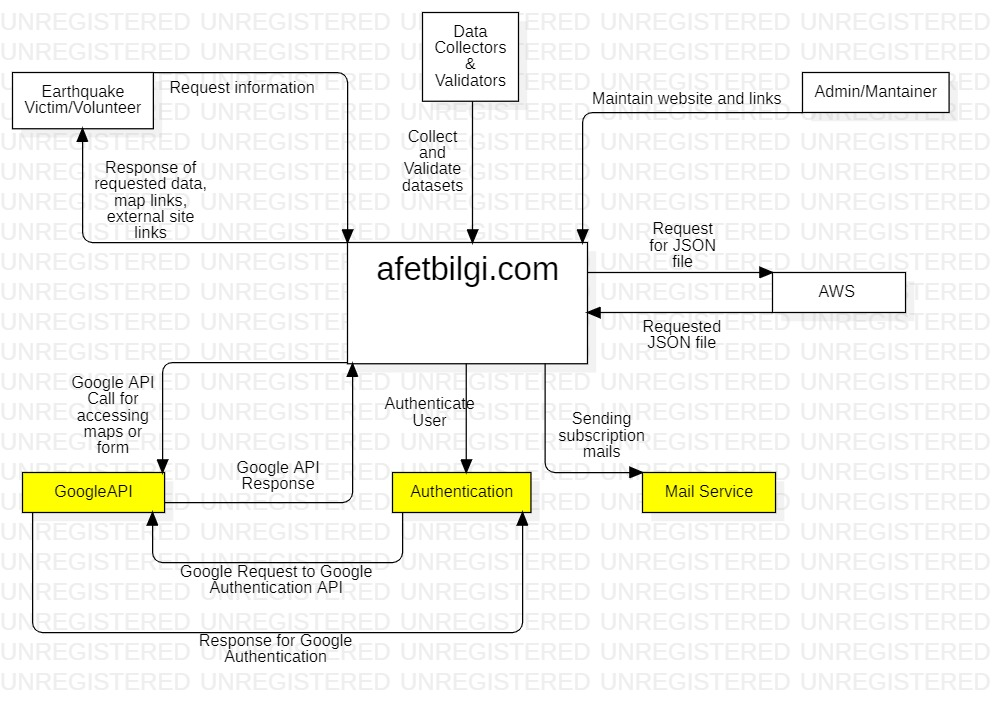
\includegraphics[width=\linewidth]{img/context-diagram-s5.jpg}
  \caption{Suggested Context Diagram}
\end{figure}

The afetbilgi.com consists of a combination of small physical and software parts. With the help of interfaces, these parts communicate among themselves and with the user.

\subsubsection{External Interfaces}

\begin{figure}[H]
  \centering
  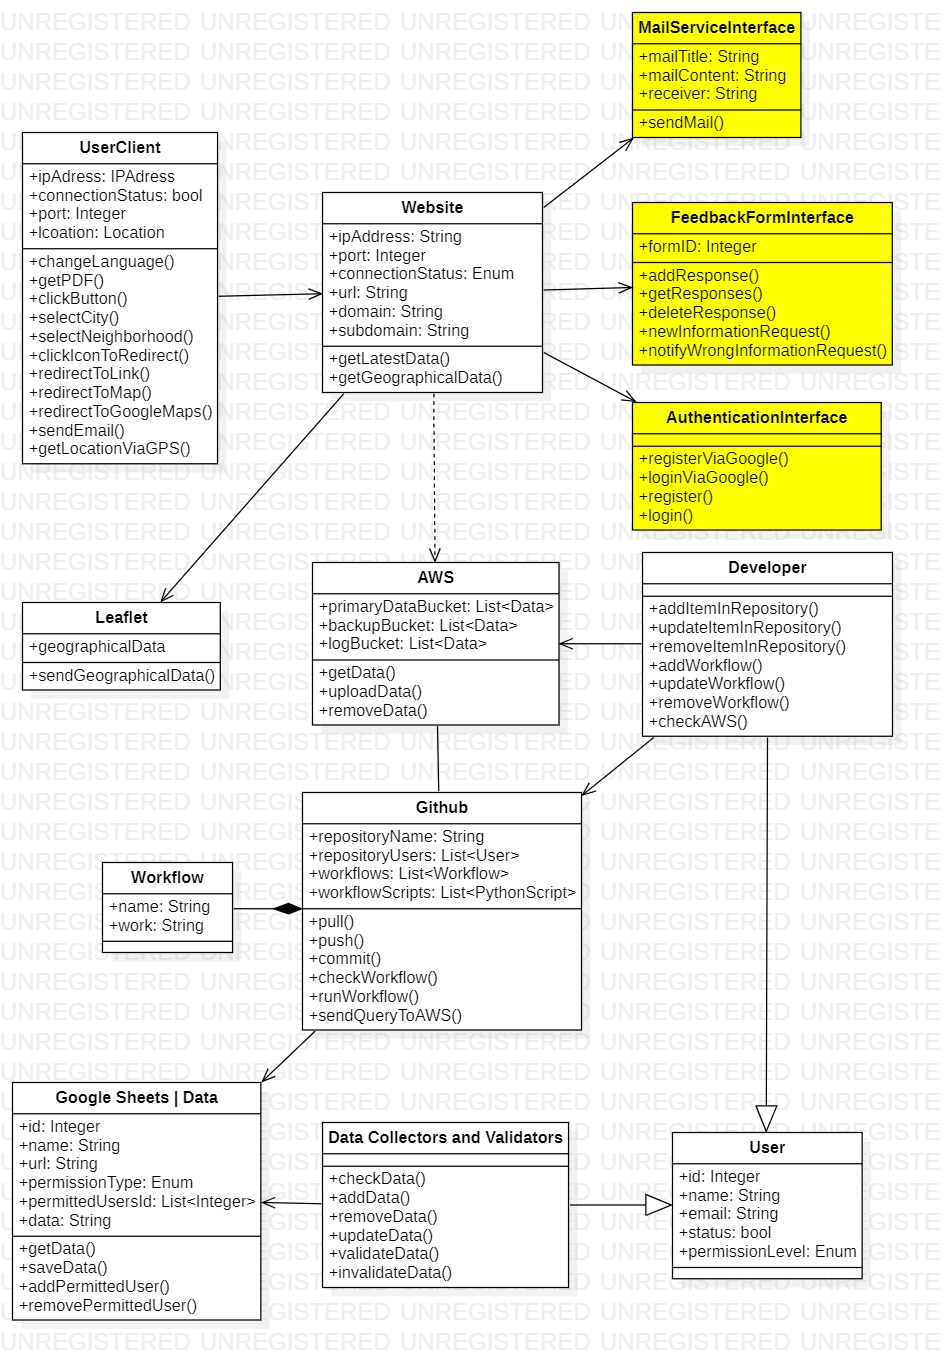
\includegraphics[width=\linewidth]{img/external-interfaces-diagram-s5.jpg}
  \caption{Suggested External Interfaces Diagram}
\end{figure}

As it can be observed from Figure \addnumbertofigure{0}, \afetbilgi has multiple external interfaces. We have added MailServiceInterface, FeedbackFormInterface and AuthenticationInterface. The operations given in the diagram can be summarized as follows:
\begin{itemize}
  \item MailServiceInterface provides the option of sending mail about the updated information to the subscribed users.
  \item FeedbackFormInterface provides the option of sending feedback related to website and the data. Users from the earthquake region can request for adding new information and notifying the wrong and expired infromation.
  \item AuthenticationInterface provides the option of logging in. The authentication system is used to provide opportunity to authorized institutions and organizations to update the information from the website directly.
\end{itemize}

\subsubsection{Interaction Scenarios}

\begin{figure}[H]
  \centering
  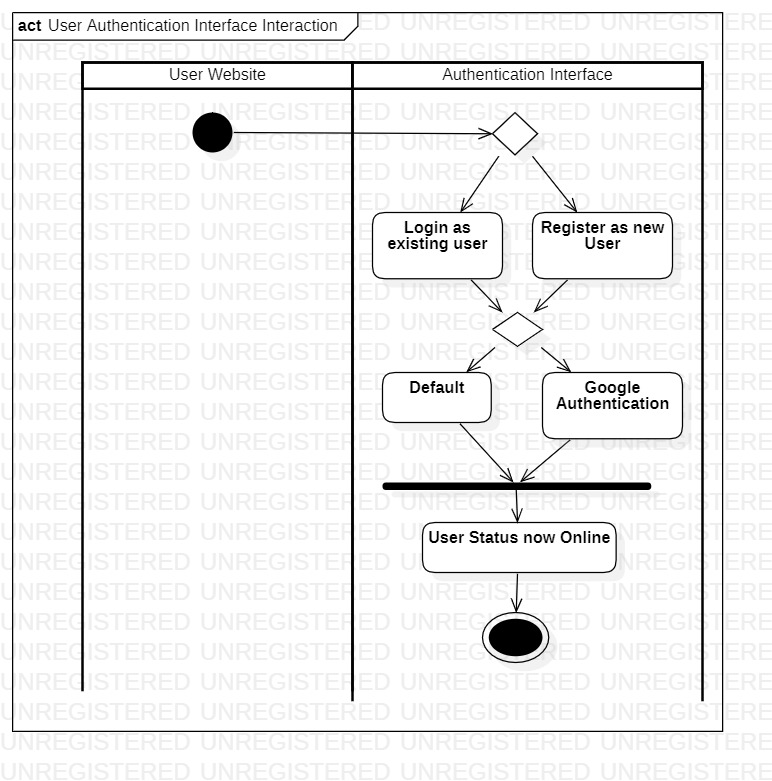
\includegraphics[width=\linewidth]{img/activity-diagram-1-s5.jpg}
  \caption{Activity Diagram | User Authentication Interface Interaction}
\end{figure}

\subsection{Functional View}

\subsubsection{Stakeholders' Uses of This View}

This view illustrates the system's various components and their interactions, including internal interfaces. Stakeholders find this view crucial as it provides information about the system's functionalities, essential properties, and supports the development of other viewpoints and diagrams. Victims and volunteers may not find this view useful, but website maintainers and data collectors would greatly appreciate it as it helps them understand the internal components and potentially identify ways to enhance them.

\subsubsection{Component Diagram}

\begin{figure}[H]
  \centering
  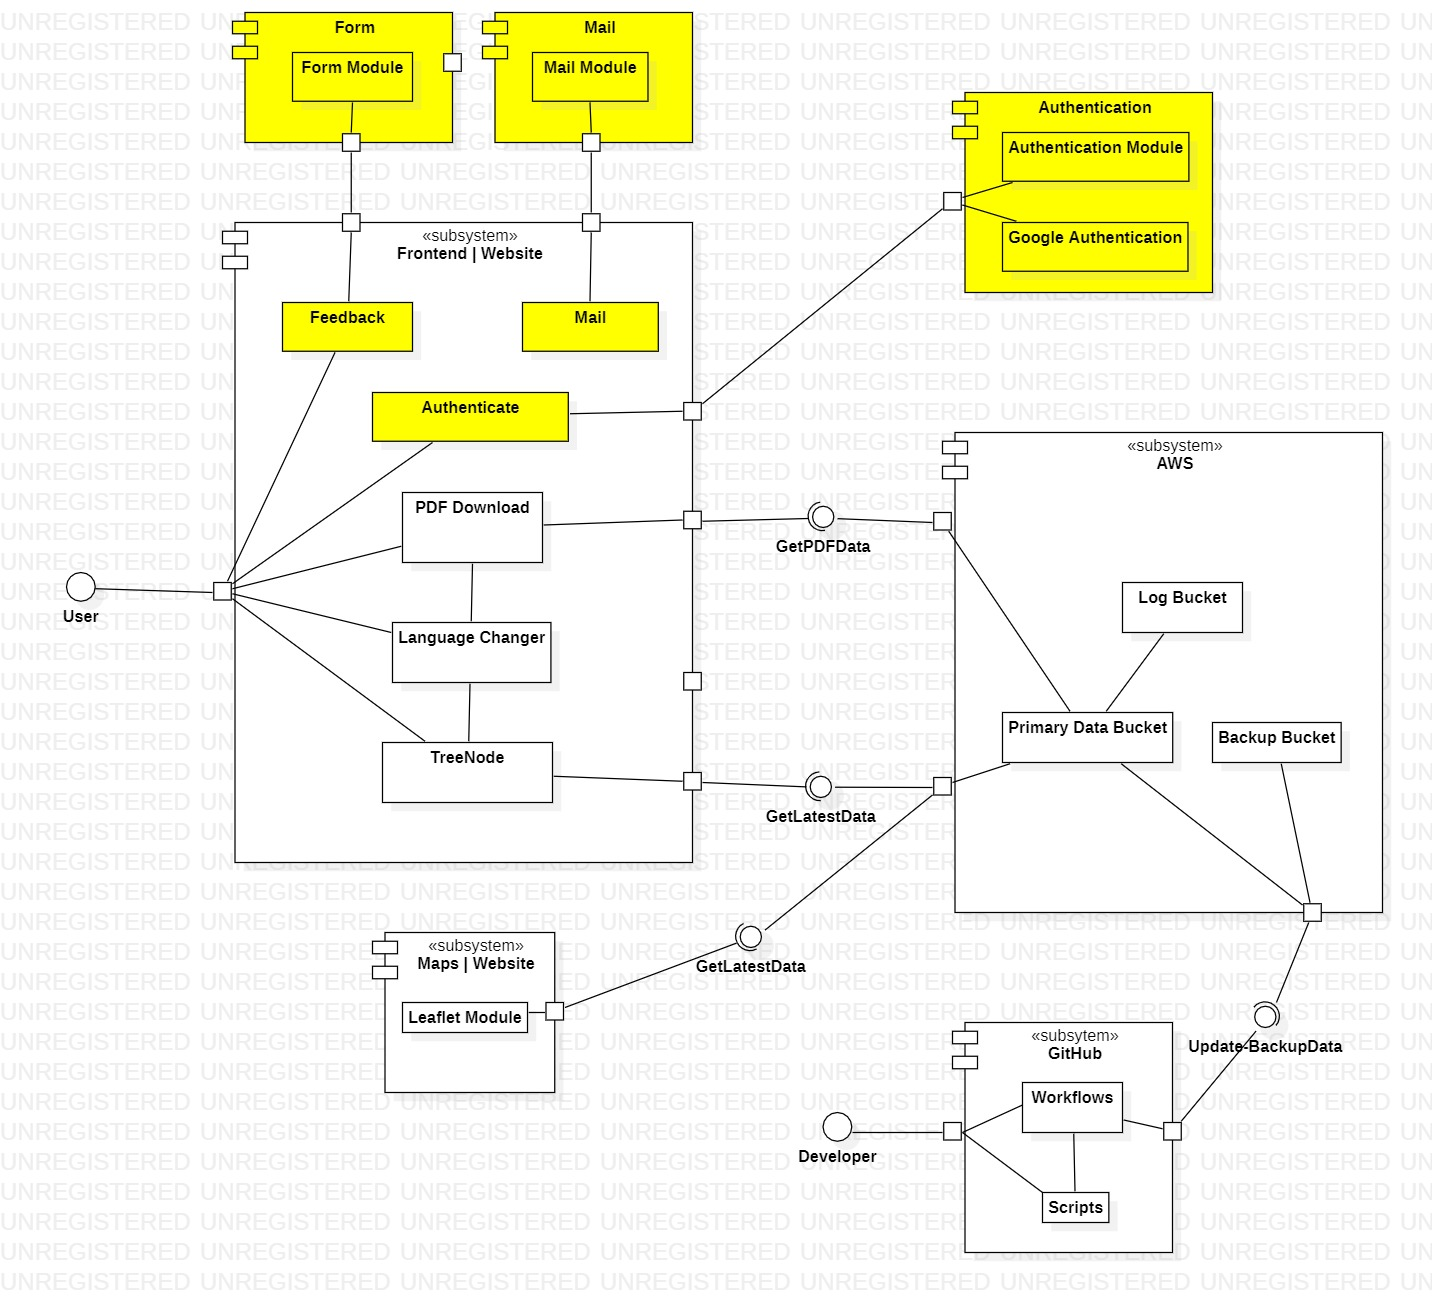
\includegraphics[width=\linewidth]{img/component-diagram-s5.jpg}
  \caption{Suggested Component Diagram}
\end{figure}

We have updated component diagram by adding the components for form, mail and authentication components:
\begin{itemize}
  \item Form provides user to send feedback about website and data so that the website and data can be updated according to the feedback by the normal users and victims.
  \item Mail component sends mail about the updated information to the subscribed users.
  \item Authentication component provide authorized users to register and login to the website by using Google Authentication system or built-in Authentication Module.
\end{itemize}

\subsubsection{Internal Interfaces}

\begin{figure}[H]
  \centering
  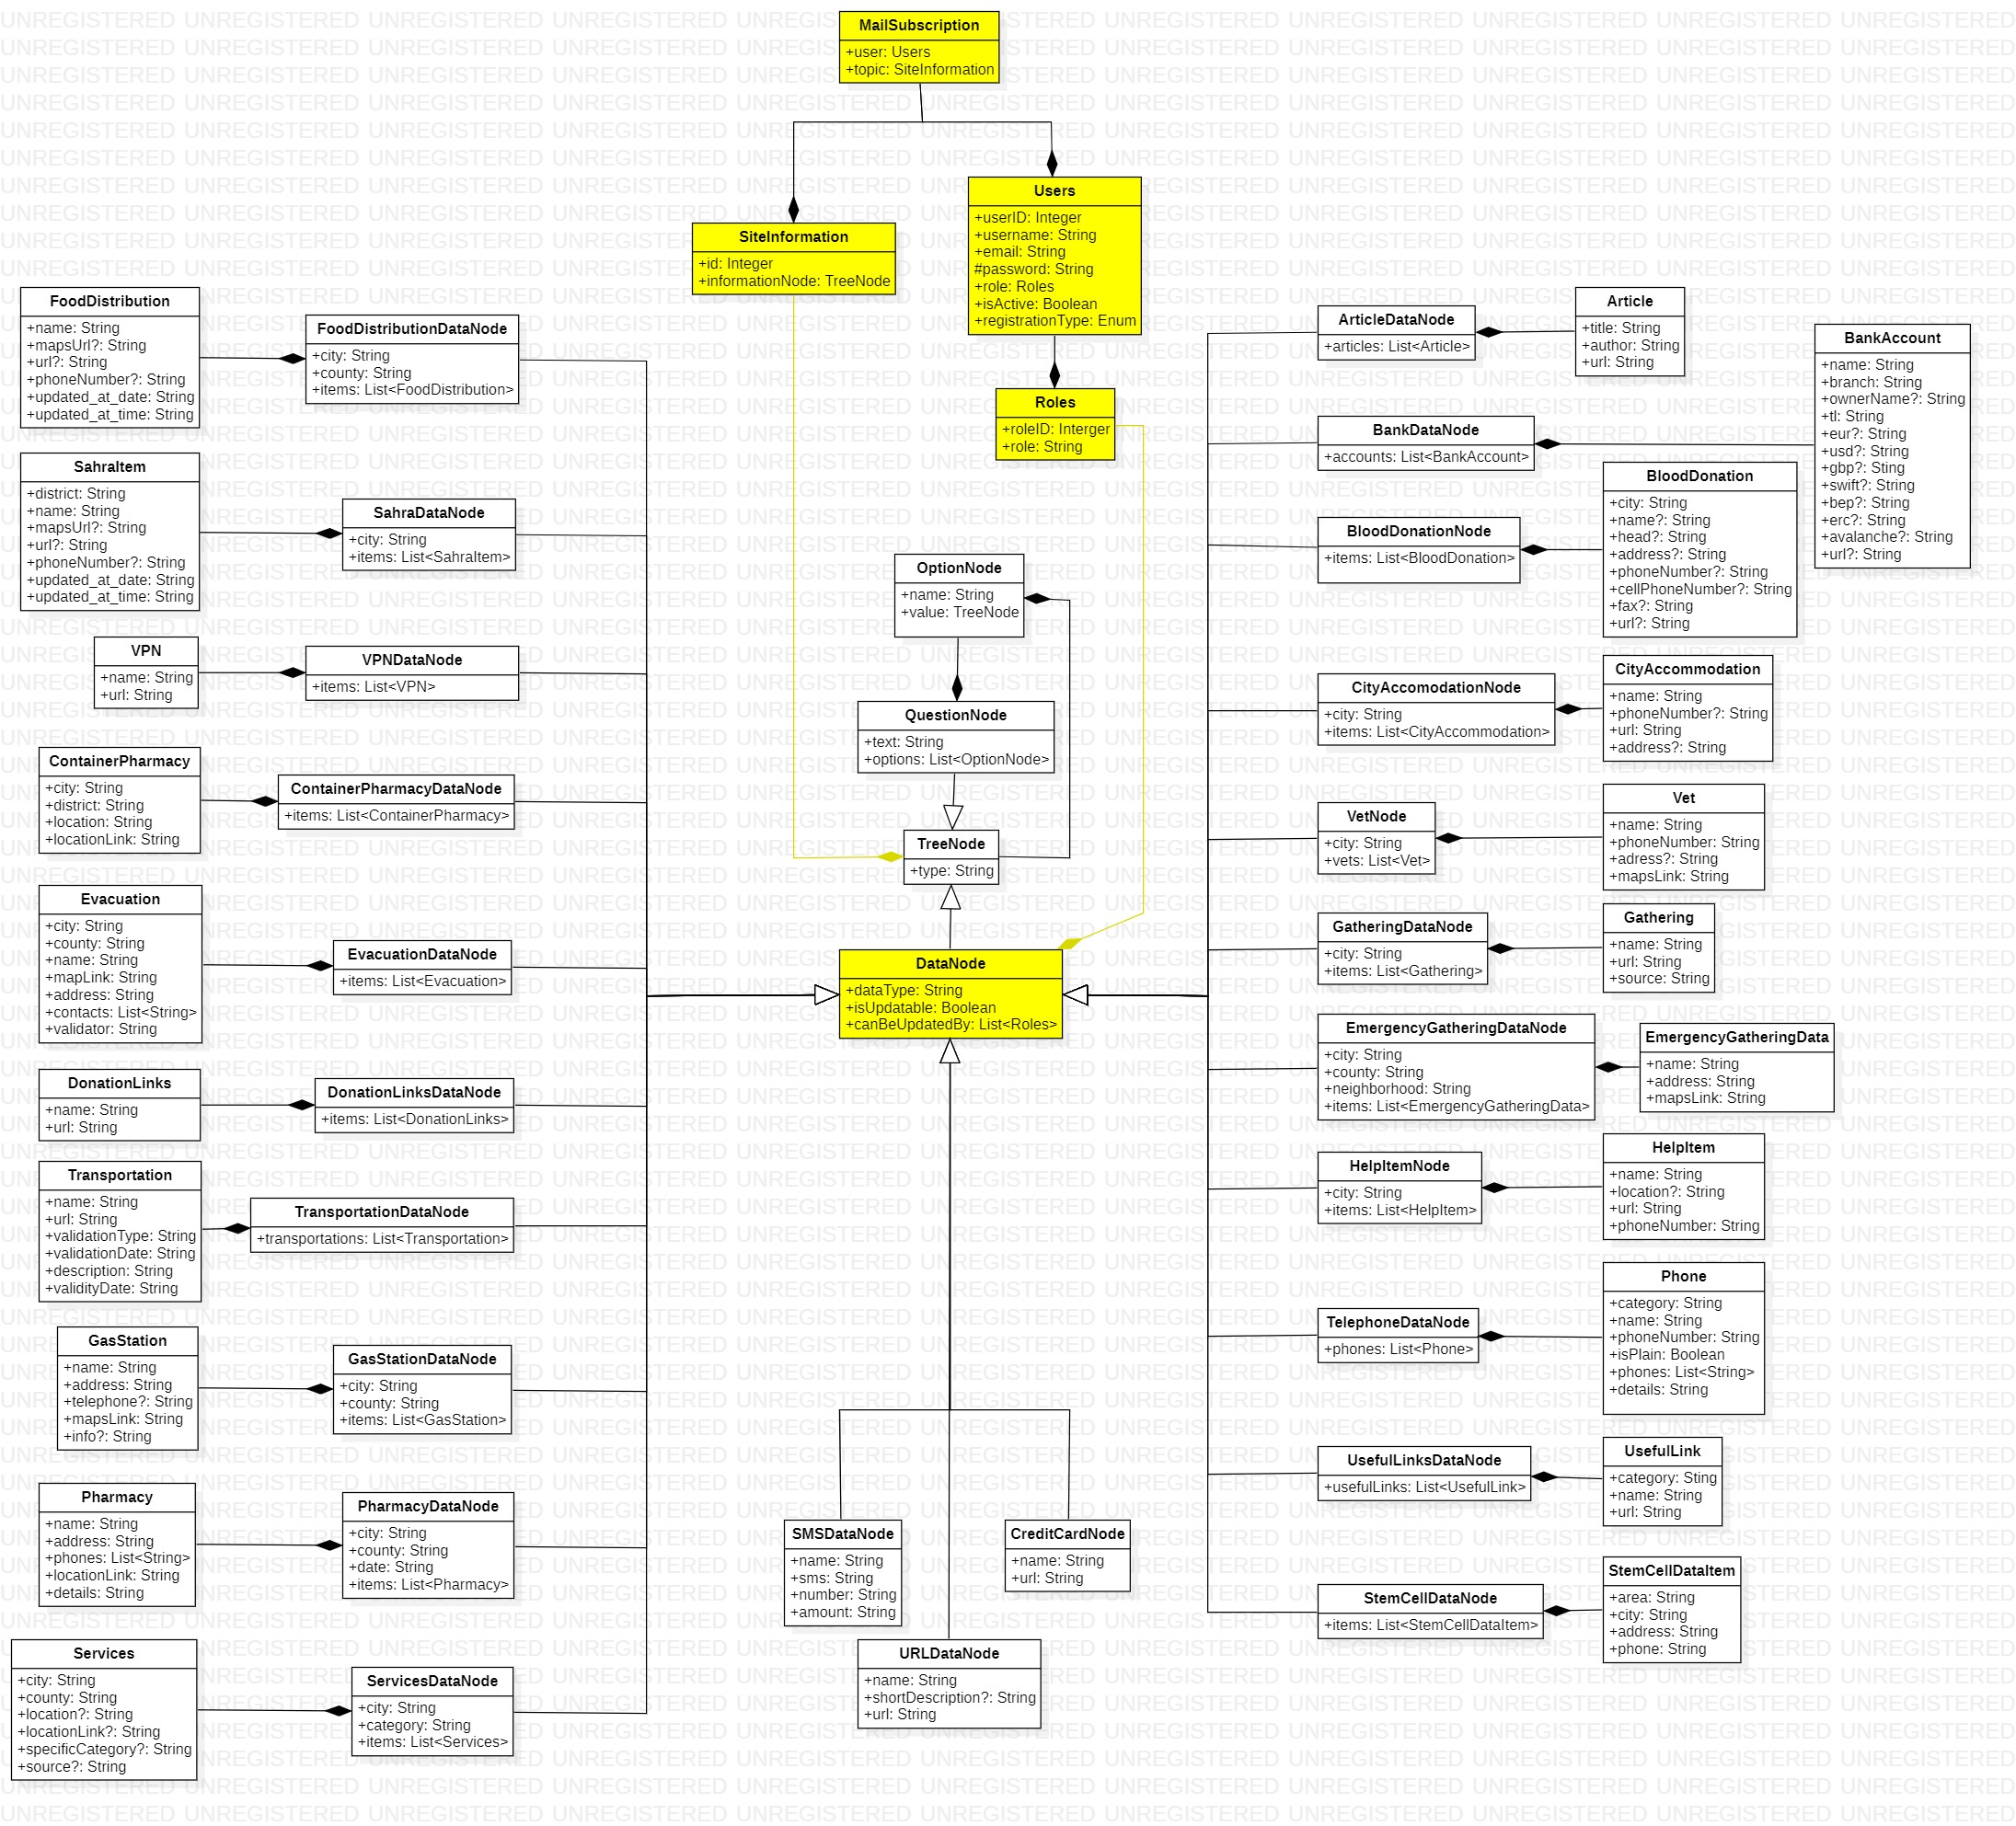
\includegraphics[width=\linewidth]{img/internal-interfaces-diagram-s5.jpg}
  \caption{Suggested Internal Interfaces}
\end{figure}


Since, there is no internal dynamism between interfaces initially, we embraced the same approches. Therefore, the internal interfaces are just the data interfaces to provide structured information for frontend code so that frontend code can parse the information correctly and fastly.

The main data is stored in the database and retrieved from database, so the frontend code parses the data.

\subsubsection{Interaction Patterns}

\begin{figure}[H]
  \centering
  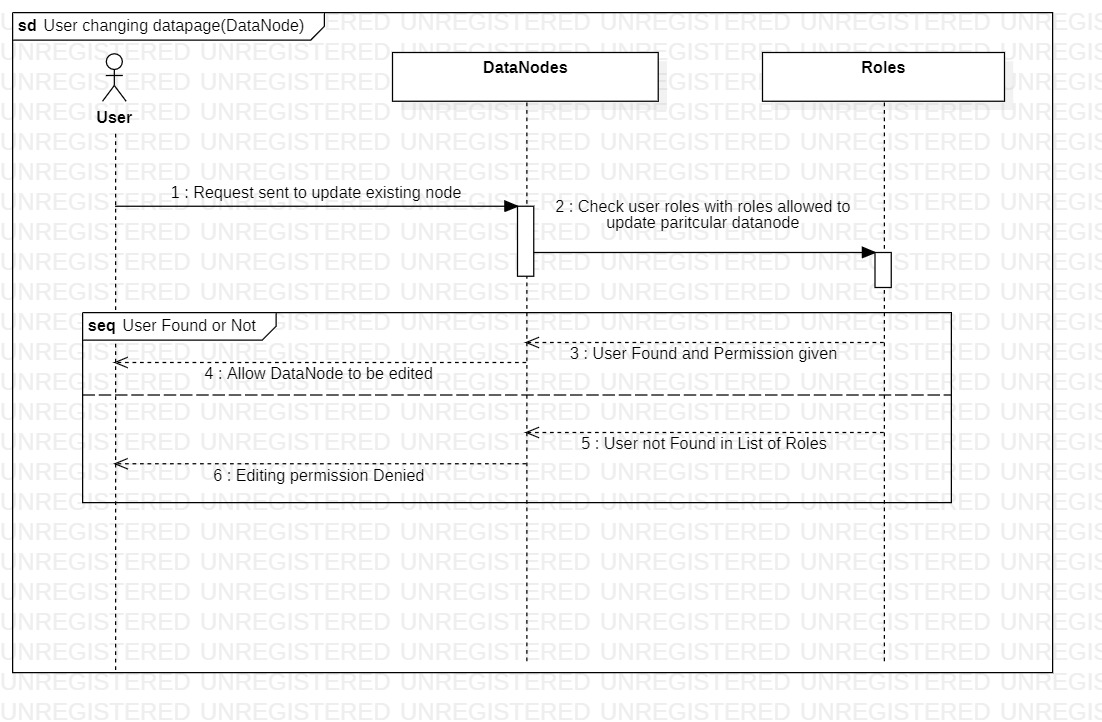
\includegraphics[width=\linewidth]{img/sequence-diagram-1-s5.jpg}
  \caption{Sequence Diagram | User Changing Datapage}
\end{figure}

\subsection{Information View}

\subsubsection{Stakeholders' Uses of This View}

The information view focuses on the variables and data utilized and stored within the system during its operation, as per Rozanski's explanations. Although this open-source, static, and non-dynamic website does not employ a database infrastructure backend like mySQL, stakeholders such as website maintainers and data maintainers/validators would still find value in knowing which data pages and nodes are being exchanged. It allows them to identify any unreliable information being uploaded to the website's assets and datasheets.

\subsubsection{Database Class Diagram}

\begin{figure}[H]
  \centering
  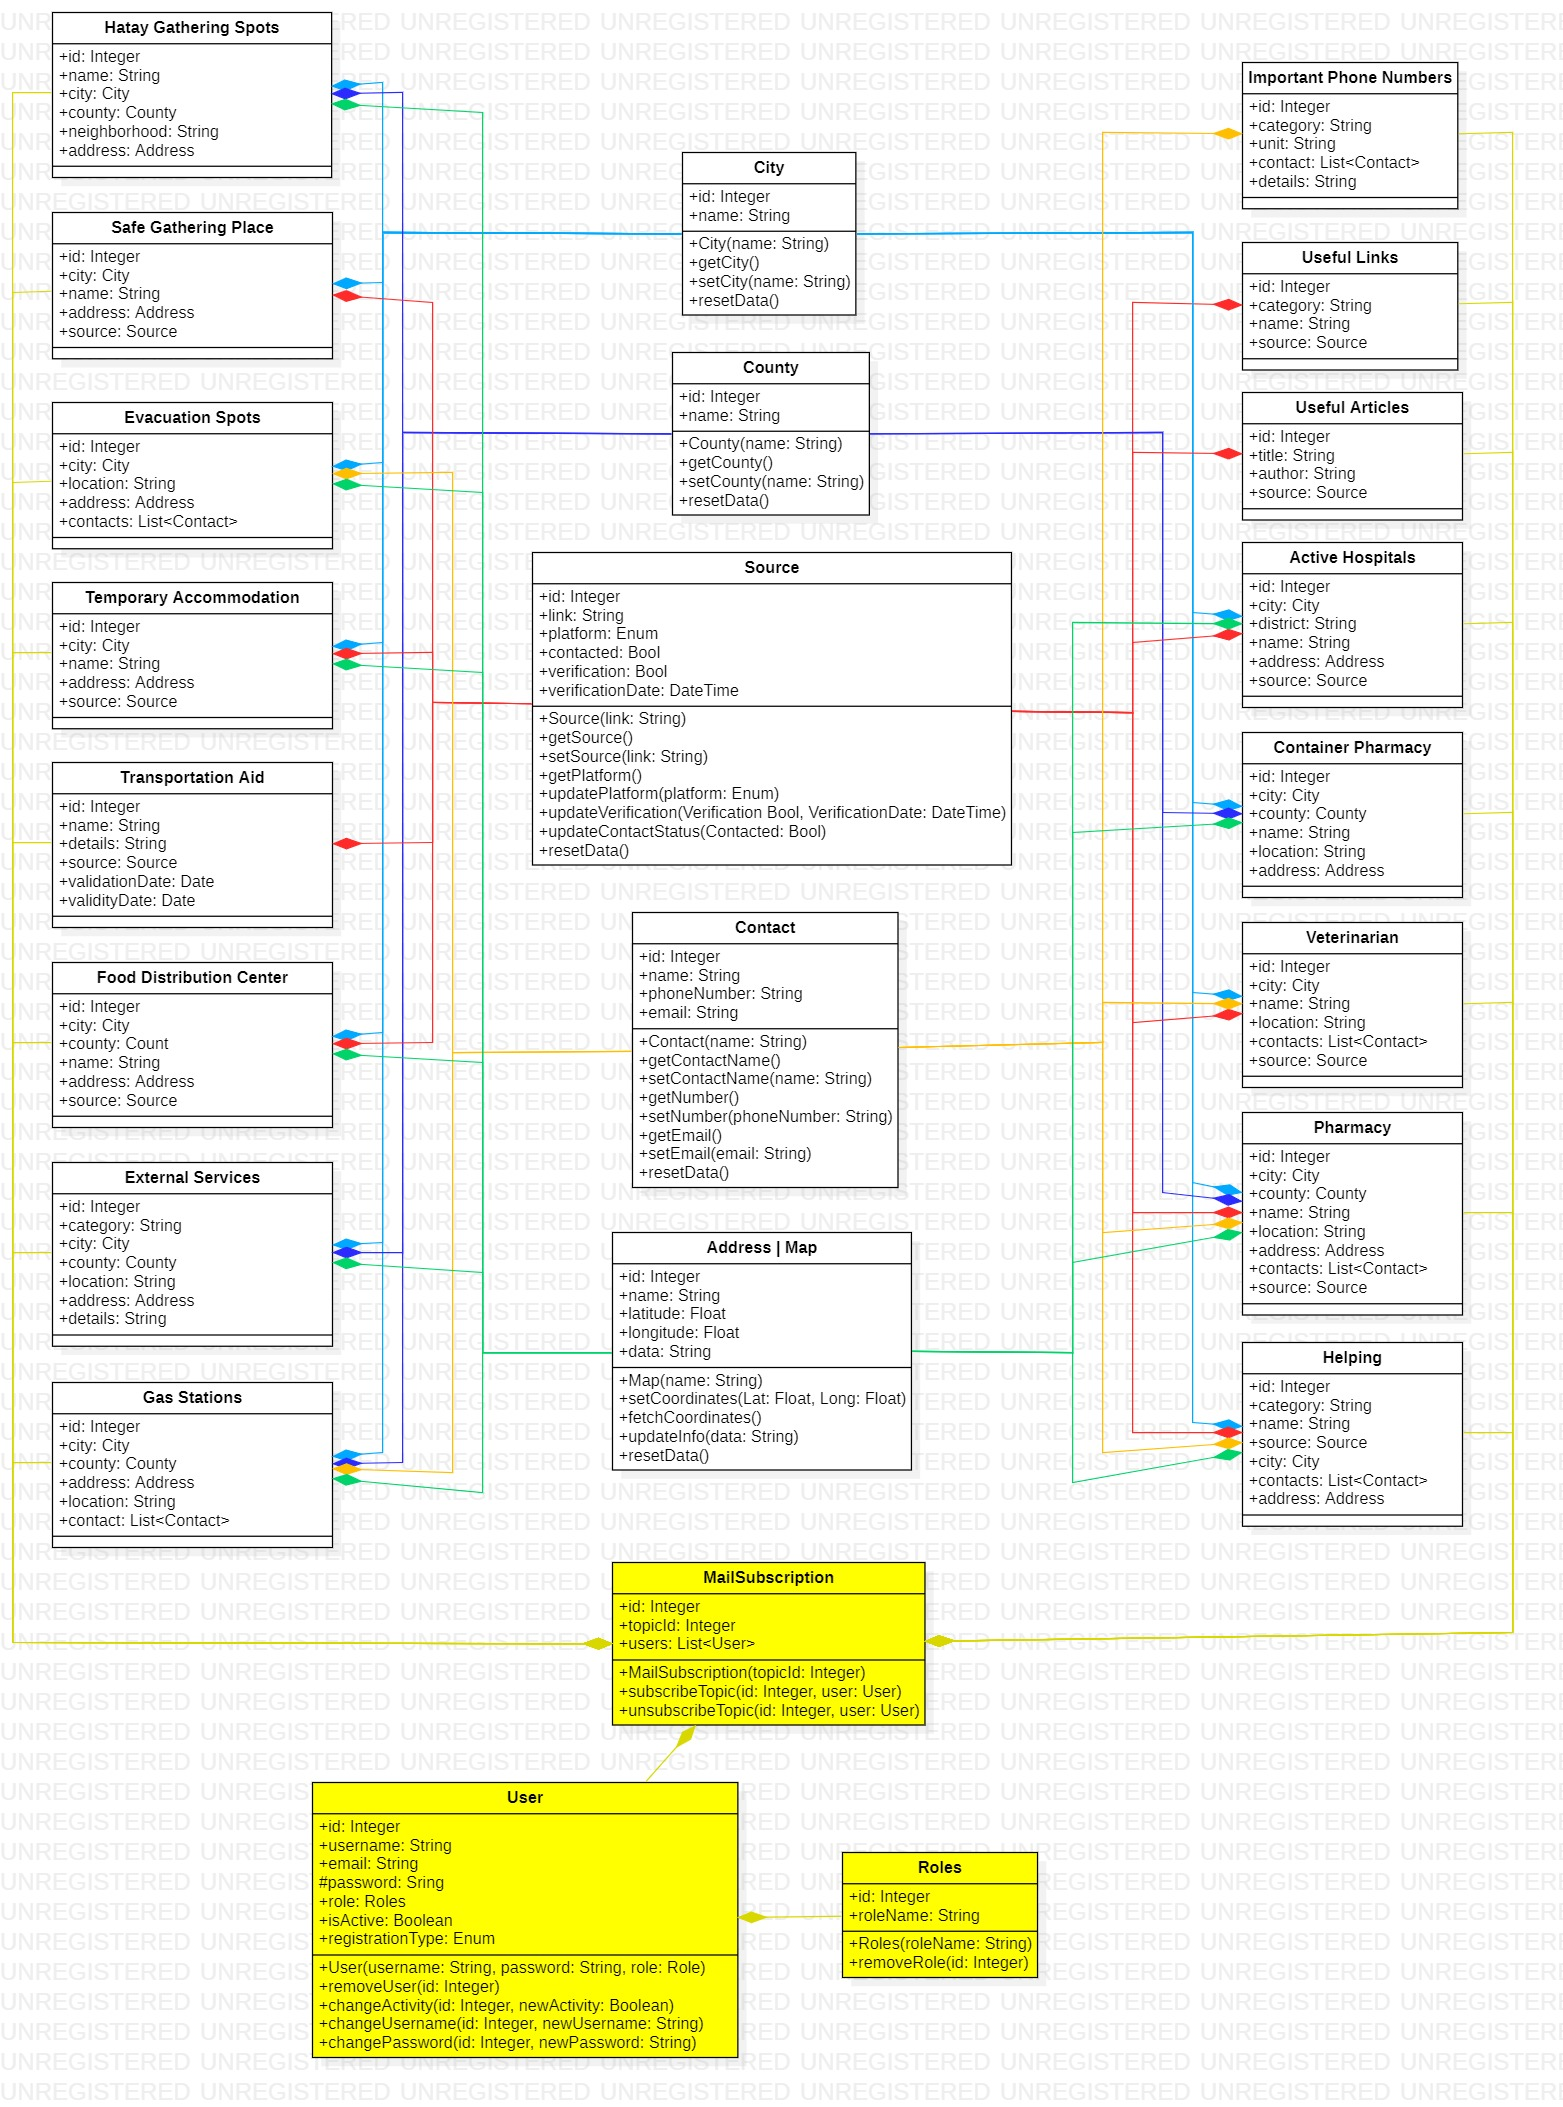
\includegraphics[width=\linewidth]{img/database-class-diagram-s5.jpg}
  \caption{Suggested Database Class Diagram}
\end{figure}

\subsubsection{Operations on Data}

\begin{longtable}{|p{.3\linewidth}|p{.7\linewidth}|}
    \hline
    Operation & CRUD Operation \\ \hline
    City::City() & Create: City Profile with name \\
               & Read: \\
               & Update: \\
               & Delete: \\ \hline
    City:: getCity() & Create: \\
                     & Read: City for selection \\
                     & Update: \\
                     & Delete: \\ \hline
    





    % Burak's Part
    MailSubscription :: MailSubscription() & Create: Create new MailSubscription item with given topicId \\
                                         & Read: \\
                                         & Update: \\
                                         & Delete: \\ \hline
    MailSubscription :: subscribeTopic() & Create: \\
                                       & Read: \\
                                       & Update: Add user to the users list of the subcription item \\
                                       & Delete: \\ \hline
    MailSubscription :: unsubscribeTopic() & Create: \\
                                         & Read: \\
                                         & Update: Remove user from the users list of the subcription item \\
                                         & Delete: \\ \hline

    User :: User() & Create: Create new user with given arguments \\
                 & Read: \\
                 & Update: \\
                 & Delete \\ \hline
    User :: removeUser() & Create: \\
                       & Read: \\
                       & Update: \\
                       & Delete: Delete user with given id \\ \hline
    User :: changeActivity() & Create: \\
                           & Read: \\
                           & Update: Update the activity status of the user \\
                           & Delete: \\ \hline
    User :: changeUsername() & Create: \\
                           & Read: \\
                           & Update: Update the username of the user \\
                           & Delete: \\ \hline
    User :: changePassword() & Create: \\
                           & Read: \\
                           & Update: Update the password of the user \\
                           & Delete: \\ \hline

    Roles :: Roles() & Create: Create new role with the given name \\
                   & Read: \\
                   & Update: \\
                   & Delete: \\ \hline
    Roles :: removeRole() & Create: \\
                        & Read: \\
                        & Update: \\
                        & Delete: Remove the role with given integer \\ \hline
  \caption{CRUD Operations on Data}
\end{longtable}

\subsection{Deployment View}

\subsubsection{Stakeholders' Uses of This View}

According to Rozanski's document, the deployment view represents the system's runtime environment, including hardware and external server elements. In the case of this project, website maintainers/admins would benefit from a basic understanding of the deployment diagram, such as running parser script files and setting up hot/cold sheets that are regularly updated to the latest.json file via the AWS S3 bucket. Additionally, future/long-term site maintainers would delve deeper into the deployment diagram to focus on individual components and enhance specific aspects, such as improving the security of coldsheets' static JSON files before merging them into the recent latest.json files.

\subsubsection{Deployment Diagram}

\begin{figure}[H]
  \centering
  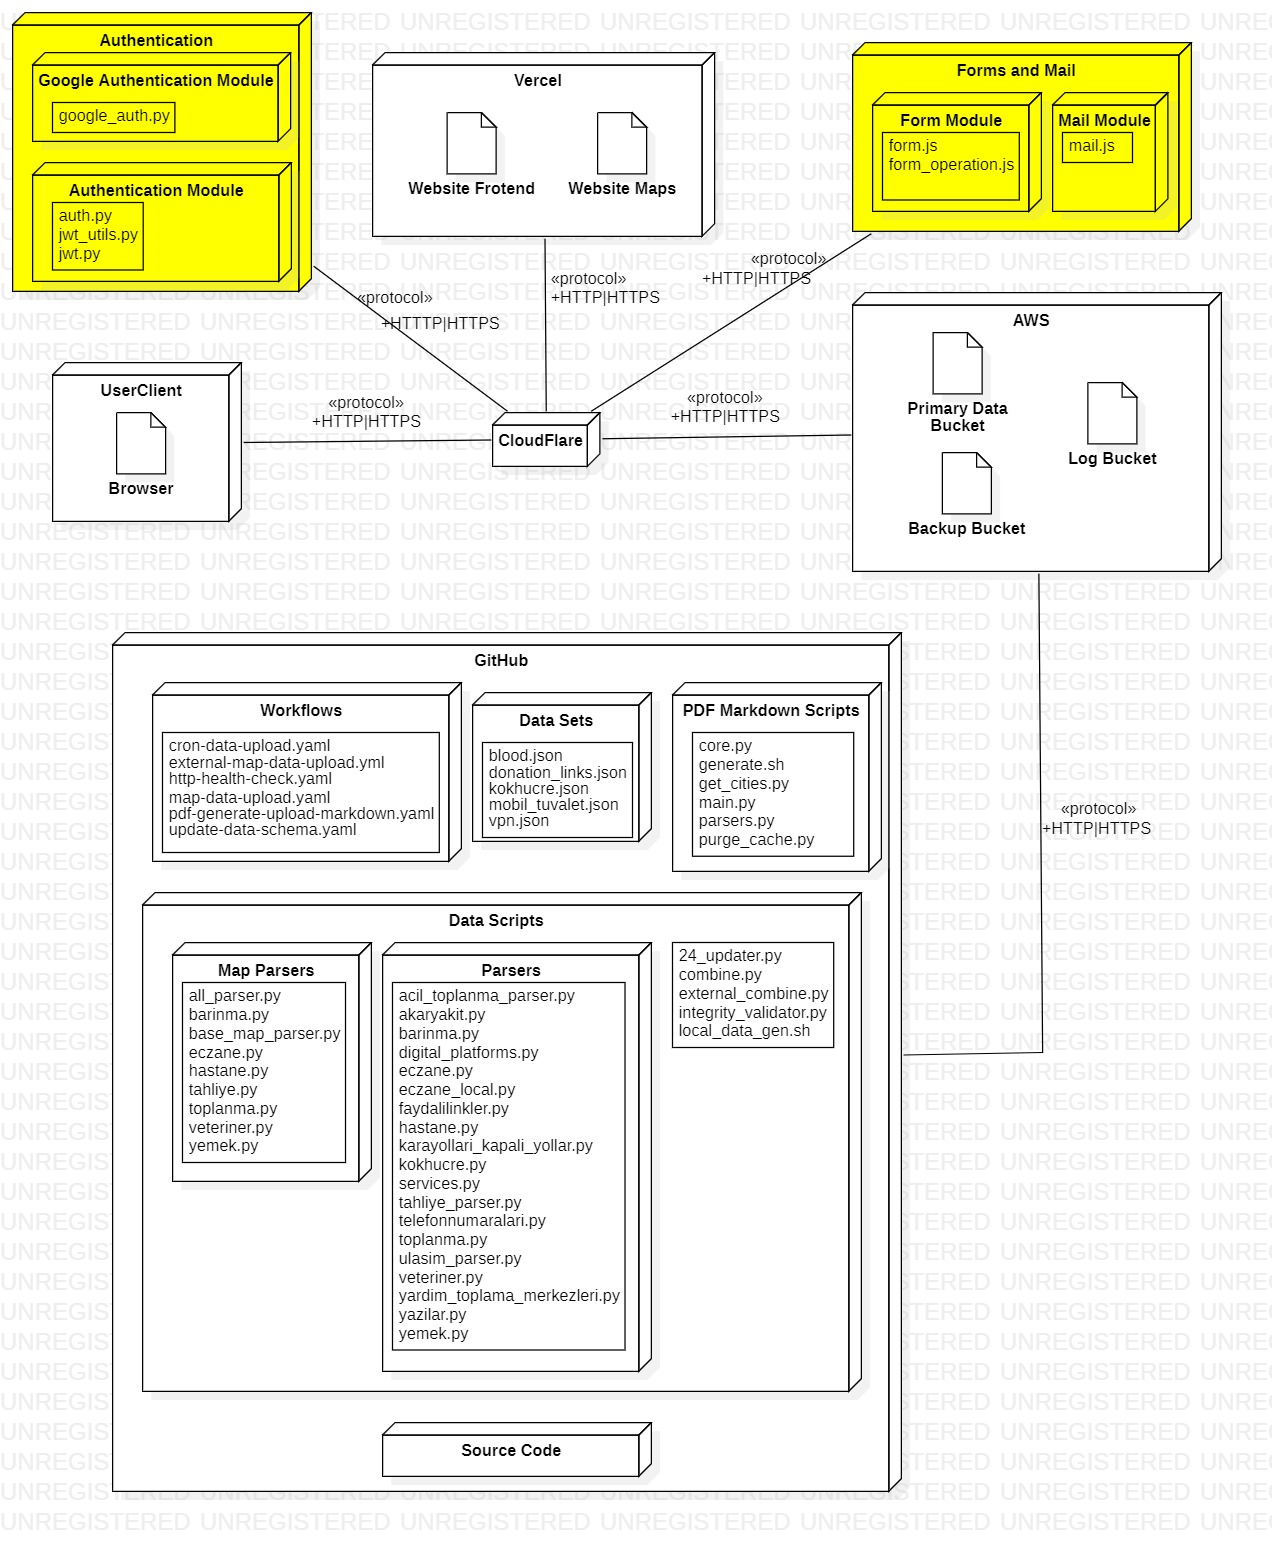
\includegraphics[width=\linewidth]{img/deployment-diagram-s5.jpg}
  \caption{Suggested Deployment Diagram}
\end{figure}

\begin{itemize}
  \item Authentication provides authorized users to register and login. It uses two systems which are Google Authentication and built-in Authentication System.
  \subitem Google Authentication access the Google API for authentication. Built-in authentication system use stored database information with JSON Web Tokens (JWT) for token based authentication system.
  \item Form provides user to send feedback about website and data. Forms to provide feedbacks are defined according to needs. Some operations such as uploading image as well as the basic form operations such as submitting.
  \item Mail modeule sends mails if there is an update in the website.
\end{itemize}

\subsection{Design Rationale}
